\section{Pruebas en Tierra}

Para validar experimentalmente la integridad estructural, la estabilidad aerodinámica y la confiabilidad del sistema de recuperación antes del vuelo oficial, el equipo ejecutó una serie de pruebas rigurosas en el laboratorio de la institución.

\subsection{Pruebas de Estabilidad Estática y Dinámica}
Conforme a las normativas del DCP 2026 y de la National Association of Rocketry (NAR), se aplicaron dos metodologías experimentales independientes para verificar la posición del Centro de Presión ($CP$) y corroborar el margen estático mínimo de 2,0 calibres frente al Centro de Gravedad medido ($CG = 38,2\text{ cm}$):

\begin{enumerate}[leftmargin=1.5em]
    \item \textbf{Método del Recorte de Cartón (Silueta Bidimensional):} Se reprodujo la silueta lateral a escala 1:1 del cohete sobre cartón rígido homogéneo y se suspendió mediante un hilo y plomada sobre una arista delgada para ubicar su centro de masa geométrico plano. Este método arroja una aproximación conservadora del Centro de Presión lateral ($CP_{\text{recorte}} = \mathbf{46,8\text{ cm}}$ desde el vértice).
    \item \textbf{Prueba Dinámica de Balanceo (Swing Test):} Con el cohete en masa final de despegue (528 g, incluyendo motor simulado e instrumentación), se ató un cordón en la posición exacta del $CG$ real ($38,2\text{ cm}$) y se procedió a balancear el vehículo en círculos horizontales a una velocidad tangencial superior a 8 m/s. El cohete mantuvo su eje apuntando firmemente hacia la dirección de avance sin oscilaciones divergentes ni cabeceo, confirmando estabilidad aerodinámica dinámica positiva.
\end{enumerate}

\begin{figure}[H]
\centering
\begin{subfigure}[b]{0.48\linewidth}
    \centering
    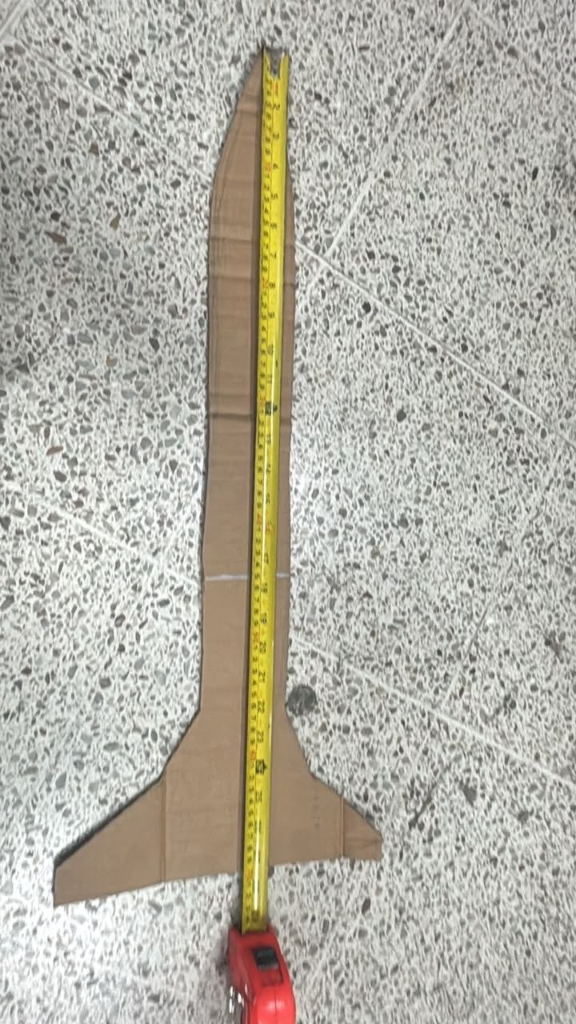
\includegraphics[width=\linewidth]{estabilidad_recorte.png}
    \caption{Determinación experimental del $CP$ mediante el método del recorte de cartón.}
    \label{fig:estabilidad_recorte}
\end{subfigure}
\hfill
\begin{subfigure}[b]{0.48\linewidth}
    \centering
    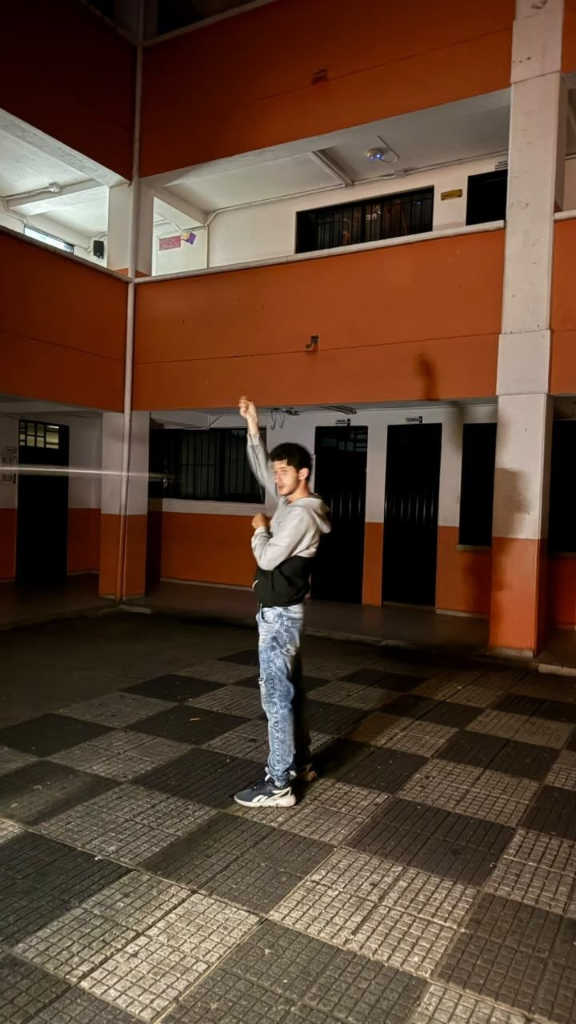
\includegraphics[width=\linewidth]{estabilidad_swing.png}
    \caption{Prueba dinámica de balanceo con cuerda (Swing Test).}
    \label{fig:estabilidad_swing}
\end{subfigure}
\caption{Ensayos experimentales de estabilidad aerodinámica en tierra.}
\label{fig:pruebas_estabilidad}
\end{figure}

\begin{table}[H]
\centering
\small
\begin{tabularx}{\linewidth}{p{4.2cm}p{3.6cm}p{3.4cm}X}
\toprule
\rowcolor{navyiejaga!15}
\textbf{Parámetro de Estabilidad} & \textbf{Valor Simulado (OpenRocket)} & \textbf{Valor Experimental} & \textbf{Estado / Cumplimiento} \\
\midrule
Centro de Gravedad ($CG$) & 38,2 cm & 38,2 cm & Medido en rampa (528 g) \\
\rowcolor{grisclaro}
Centro de Presión ($CP$) & 51,4 cm (Barrowman) & 46,8 cm (Recorte) & Verificado experimentalmente \\
Separación estática ($CP - CG$) & 13,2 cm & 8,6 cm & Margen estático positivo \\
\rowcolor{grisclaro}
\textbf{Margen de estabilidad} & \textbf{2,00 calibres} & \textbf{2,00 calibres} & \textbf{Aprobado} (Norma: $\ge 2,0\text{ cal}$) \\
\bottomrule
\end{tabularx}
\caption{Comparación de parámetros de estabilidad teóricos frente a mediciones experimentales.}
\label{tab:comparacion_estabilidad}
\end{table}

\subsection{Pruebas de Despliegue de Recuperación y Banco de Aviónica}
Se realizaron ensayos de eyección en banco mediante sobrepresión neumática manual en el fuselaje, verificando que la ojiva y la bahía de carga útil se desacoplan suavemente sin atascamientos mecánicos cuando la manta Nomex y el paracaídas de 40 cm están debidamente plegados en su compartimento.

Asimismo, la aviónica de la carga útil fue sometida a pruebas de vibración mecánica sostenida durante 48 segundos para certificar la ausencia de falsos contactos en los terminales de la batería NiMH y la resistencia a la aceleración de la tarjeta microSD.

% Placeholder para fotografía de prueba de eyección en banco si el equipo desea incluirla
\placeholderbox{figures/prueba_eyeccion_banco.png}{Ensayo de sobrepresión neumática y eyección en banco del paracaídas de 40 cm.}
